\documentclass[12pt,]{article}
\usepackage{lmodern}
\usepackage{amssymb,amsmath}
\usepackage{ifxetex,ifluatex}
\usepackage{fixltx2e} % provides \textsubscript
\ifnum 0\ifxetex 1\fi\ifluatex 1\fi=0 % if pdftex
  \usepackage[T1]{fontenc}
  \usepackage[utf8]{inputenc}
\else % if luatex or xelatex
  \ifxetex
    \usepackage{mathspec}
  \else
    \usepackage{fontspec}
  \fi
  \defaultfontfeatures{Ligatures=TeX,Scale=MatchLowercase}
\fi
% use upquote if available, for straight quotes in verbatim environments
\IfFileExists{upquote.sty}{\usepackage{upquote}}{}
% use microtype if available
\IfFileExists{microtype.sty}{%
\usepackage{microtype}
\UseMicrotypeSet[protrusion]{basicmath} % disable protrusion for tt fonts
}{}
\usepackage[margin=1in]{geometry}
\usepackage{hyperref}
\hypersetup{unicode=true,
            pdfauthor={Xuan Son Le (4669361), Freie Universität Berlin},
            pdfborder={0 0 0},
            breaklinks=true}
\urlstyle{same}  % don't use monospace font for urls
\usepackage{color}
\usepackage{fancyvrb}
\newcommand{\VerbBar}{|}
\newcommand{\VERB}{\Verb[commandchars=\\\{\}]}
\DefineVerbatimEnvironment{Highlighting}{Verbatim}{commandchars=\\\{\}}
% Add ',fontsize=\small' for more characters per line
\usepackage{framed}
\definecolor{shadecolor}{RGB}{248,248,248}
\newenvironment{Shaded}{\begin{snugshade}}{\end{snugshade}}
\newcommand{\KeywordTok}[1]{\textcolor[rgb]{0.13,0.29,0.53}{\textbf{#1}}}
\newcommand{\DataTypeTok}[1]{\textcolor[rgb]{0.13,0.29,0.53}{#1}}
\newcommand{\DecValTok}[1]{\textcolor[rgb]{0.00,0.00,0.81}{#1}}
\newcommand{\BaseNTok}[1]{\textcolor[rgb]{0.00,0.00,0.81}{#1}}
\newcommand{\FloatTok}[1]{\textcolor[rgb]{0.00,0.00,0.81}{#1}}
\newcommand{\ConstantTok}[1]{\textcolor[rgb]{0.00,0.00,0.00}{#1}}
\newcommand{\CharTok}[1]{\textcolor[rgb]{0.31,0.60,0.02}{#1}}
\newcommand{\SpecialCharTok}[1]{\textcolor[rgb]{0.00,0.00,0.00}{#1}}
\newcommand{\StringTok}[1]{\textcolor[rgb]{0.31,0.60,0.02}{#1}}
\newcommand{\VerbatimStringTok}[1]{\textcolor[rgb]{0.31,0.60,0.02}{#1}}
\newcommand{\SpecialStringTok}[1]{\textcolor[rgb]{0.31,0.60,0.02}{#1}}
\newcommand{\ImportTok}[1]{#1}
\newcommand{\CommentTok}[1]{\textcolor[rgb]{0.56,0.35,0.01}{\textit{#1}}}
\newcommand{\DocumentationTok}[1]{\textcolor[rgb]{0.56,0.35,0.01}{\textbf{\textit{#1}}}}
\newcommand{\AnnotationTok}[1]{\textcolor[rgb]{0.56,0.35,0.01}{\textbf{\textit{#1}}}}
\newcommand{\CommentVarTok}[1]{\textcolor[rgb]{0.56,0.35,0.01}{\textbf{\textit{#1}}}}
\newcommand{\OtherTok}[1]{\textcolor[rgb]{0.56,0.35,0.01}{#1}}
\newcommand{\FunctionTok}[1]{\textcolor[rgb]{0.00,0.00,0.00}{#1}}
\newcommand{\VariableTok}[1]{\textcolor[rgb]{0.00,0.00,0.00}{#1}}
\newcommand{\ControlFlowTok}[1]{\textcolor[rgb]{0.13,0.29,0.53}{\textbf{#1}}}
\newcommand{\OperatorTok}[1]{\textcolor[rgb]{0.81,0.36,0.00}{\textbf{#1}}}
\newcommand{\BuiltInTok}[1]{#1}
\newcommand{\ExtensionTok}[1]{#1}
\newcommand{\PreprocessorTok}[1]{\textcolor[rgb]{0.56,0.35,0.01}{\textit{#1}}}
\newcommand{\AttributeTok}[1]{\textcolor[rgb]{0.77,0.63,0.00}{#1}}
\newcommand{\RegionMarkerTok}[1]{#1}
\newcommand{\InformationTok}[1]{\textcolor[rgb]{0.56,0.35,0.01}{\textbf{\textit{#1}}}}
\newcommand{\WarningTok}[1]{\textcolor[rgb]{0.56,0.35,0.01}{\textbf{\textit{#1}}}}
\newcommand{\AlertTok}[1]{\textcolor[rgb]{0.94,0.16,0.16}{#1}}
\newcommand{\ErrorTok}[1]{\textcolor[rgb]{0.64,0.00,0.00}{\textbf{#1}}}
\newcommand{\NormalTok}[1]{#1}
\usepackage{graphicx,grffile}
\makeatletter
\def\maxwidth{\ifdim\Gin@nat@width>\linewidth\linewidth\else\Gin@nat@width\fi}
\def\maxheight{\ifdim\Gin@nat@height>\textheight\textheight\else\Gin@nat@height\fi}
\makeatother
% Scale images if necessary, so that they will not overflow the page
% margins by default, and it is still possible to overwrite the defaults
% using explicit options in \includegraphics[width, height, ...]{}
\setkeys{Gin}{width=\maxwidth,height=\maxheight,keepaspectratio}
\IfFileExists{parskip.sty}{%
\usepackage{parskip}
}{% else
\setlength{\parindent}{0pt}
\setlength{\parskip}{6pt plus 2pt minus 1pt}
}
\setlength{\emergencystretch}{3em}  % prevent overfull lines
\providecommand{\tightlist}{%
  \setlength{\itemsep}{0pt}\setlength{\parskip}{0pt}}
\setcounter{secnumdepth}{5}
% Redefines (sub)paragraphs to behave more like sections
\ifx\paragraph\undefined\else
\let\oldparagraph\paragraph
\renewcommand{\paragraph}[1]{\oldparagraph{#1}\mbox{}}
\fi
\ifx\subparagraph\undefined\else
\let\oldsubparagraph\subparagraph
\renewcommand{\subparagraph}[1]{\oldsubparagraph{#1}\mbox{}}
\fi

%%% Use protect on footnotes to avoid problems with footnotes in titles
\let\rmarkdownfootnote\footnote%
\def\footnote{\protect\rmarkdownfootnote}

%%% Change title format to be more compact
\usepackage{titling}

% Create subtitle command for use in maketitle
\newcommand{\subtitle}[1]{
  \posttitle{
    \begin{center}\large#1\end{center}
    }
}

\setlength{\droptitle}{-2em}
  \title{\textbf{Logistische Regression}}
  \pretitle{\vspace{\droptitle}\centering\huge}
  \posttitle{\par}
  \author{Xuan Son Le (4669361), Freie Universität Berlin}
  \preauthor{\centering\large\emph}
  \postauthor{\par}
  \predate{\centering\large\emph}
  \postdate{\par}
  \date{02/04/2018}


\begin{document}
\maketitle

{
\setcounter{tocdepth}{3}
\tableofcontents
}
\textbf{Abstract:} Im Rahmen der Abschlussarbeit des Moduls
Programmieren mit R im Winter-\newline semester 2017/2018 an der Freie
Universität Berlin wird für diese Arbeit die statistische Methode namens
binäres Logit-Modell ausgewählt. Diese Arbeit besteht aus zwei großen
Hauptteilen: der Theorieteil, wobei die ausgewählte Methode theoretisch
vorgestellt wird und der Implementierungsteil, welcher die Erklärung der
Funktionalität vom selbst entwickelten Paket beinhaltet. Im Theorieteil
wird zunächst ein Überblick über die grundliegende Funktionsweise vom
(binären) Logit-Modell widergegeben. Die Grundidee von Generalisierten
linearen Modellen wird anschließend kurz eingeführt, bevor der Aufbau
vom binären Logit-Modell durch das Maximum Likelihood Verfahren
vorgenommen wird. Demzufolge folgt die Interpretation der Koeffizienten
und der Lösungsgüte vom binären Logit-Modell. Schließlich werden im
Implementierungsteil alle Funktionen vom R-Paket schritterweise
vorgestellt.

\textbf{Keywords:} \emph{Logit-Modell, logistische Regression, Paket, R}

\newpage

\section{Motivation}\label{motivation}

Die Anwendung von der klassischen linearen Regression ist für binäre
(binomiale oder dichotome) Zielvariable, welche lediglich zwei Werte
(ja/nein, mänlich/weiblich, erfolgreich/nicht erfolgreich, etc.)
annehmen kann, nicht mehr geeignet, da die Zielvariable von der linearen
Regression metrisch skaliert ist. Oft wird binäre Variable als
0/1-Variable kodiert, das heißt sie nimmt nur den Wert 0 oder 1 an. Die
folgende Grafik stellt den Ansatz graphisch dar, binäre Variable durch
lineare Regression zu modellieren:

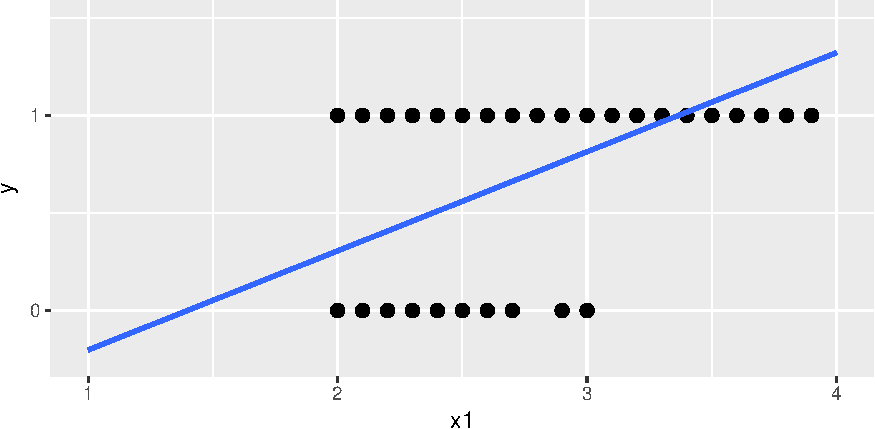
\includegraphics{logisticRegression_files/figure-latex/unnamed-chunk-1-1.pdf}

Graphisch lässt sich festlegen, dass die lineare Regression den
Wertebereich {[}0,1{]} von binären Responsevariablen sehr schnell
verlässt. Wenn die Annahmen von der linearen Regression noch in Betracht
gezogen werden, ergeben sich darüber hinaus noch folgende Probleme:

\begin{itemize}
\item
\item
\item
\end{itemize}

Aus diesen Gründen wird ein ganz anderer Ansatz benötigt, um binäre
Zielvariable zu modellieren, nämlich das binäre Logit-Modell, welches
ebenfalls als binäre logistische Regression oder binäres logistisches
Regressionsmodell bezeichnet werden kann. In der Statistik lassen sich
Logit-Modelle noch in multinomiale und kumulative Logit-Modelle
aufteilen, je nachdem ob die abhängige Variable multinominal- oder
ordinalskaliert sind . Diese Arbeit beschäftigt sich mit dem binären
Logit-Modell, welches den Zusammenhang zwischen einer binären abhängigen
Variable und einer/mehreren unabhängigen Variablen untersucht. Bei allen
Arten von Logit-Modellen können die unabhängigen Variablen beliebig
skaliert sein.

Im Unterschied zu der klassischen linearen Regression, welche den wahren
Wert einer Zielvariable vorhersagt, interessiert sich das binäre
Logit-Modell eher für die Wahrscheinlichkeit, dass die Zielvariable den
Wert 1 annimmt. Das Hauptziel vom binären Logit-Modell ist es, die
Wahrscheinlichkeit für den Eintritt der Zielvariable vorherzusagen.
Dadurch soll die folgende theoretische Fragestellung beantwortet werden:
\emph{Wie stark ist der Einfluss von den unabhängigen (erklärenden)
Variablen auf die Wahrscheinlichkeit, dass die abhängige (zu erklärende
/ Response) Variable eintritt beziehungsweise den Wert 1 annimmt?} In
der Praxis kann diese Fragestellung beispielsweise so formuliert werden:
``Haben Alter, Geschlecht, Berufe oder andere Merkmale der Kunden
Einfluss auf die Wahrscheinlichkeit, dass sie ein Kredit rechtzeitig
zurückzahlen?'' oder ``Lässt sich die Wahrscheinlichkeit, dass es
regnet, durch die Temparatur, die Windstärke oder
Sonnenstrahlungsintensität vorhersagen?''.

\section{Das binäre Logit-Modell}\label{das-binare-logit-modell}

\subsection{Modellspezifikation}\label{modellspezifikation}

Das Logit-Modell ist eine Methode aus der Algorithmenklasse namens
\emph{Generalisierte Lineare Modelle}, welche eine Verallgemeinerung des
klassischen linearen Regressionsmodells anstrebt. Dazu gehören noch die
klassische lineare Regression, Probitmodell und Poisson-Regression.

\subsection{Maximum Likelihood
Schätzung}\label{maximum-likelihood-schatzung}

Während bei der klassischen linearen Regression die Methode der
Kleinsten Quadrate (engl. \emph{method of least squares}) genutzt wird,
um die ``beste'' Regressionslinie zu bestimmen, findet

\subsection{Intepretation der
Koeffizienten}\label{intepretation-der-koeffizienten}

\section{Implementierung in R}\label{implementierung-in-r}

Im Folgenden wird die Funktionalität von dem Package \ldots{} erklärt,
welches zum Ziel setzt, die Grundidee hinter dem binären Logit-Modell
programmiert darzustellen.

Ein Beispieldatensatz wird verwendet, um die Richtigkeit und
Vollständigkeit der Ergebnisse der implementierten Methode im Vergleich
zu der R-Standardmethode für Logit-Modell zu testen. Die binäre
Responsevariable heißt \emph{admit}, welche besagt ob ein Kandidat eine
Zulassung bekommt. Zudem enthält der Datensatz drei unabhängige
Variablen: \emph{gre}, \emph{gpa} (metrisch) und \emph{rank}
(kategorial). Der Datensatz soll ein Modell unterstützen, welche die
Abhängigkeit von der Wahrscheinlichkeit einer Zulassung von der
Abschlussnote, GRE-Note sowie der Ruf von der angestrebten Institution.

Das gerade ausgeführte Beispiel kann direkt in R geladen werden. Dafür
wird in das Paket ein Vignette eingebaut, so dass wenn den folgenden
Code ausgeführt wird, wird das Beispiel in der Help-Seite von R
angezeigt.

\begin{Shaded}
\begin{Highlighting}[]
\KeywordTok{setwd}\NormalTok{(}\StringTok{"~/Desktop/Uni/Master/WS1718/ProgR/Abschlussarbeit/logisticRegression/Code/logitModell"}\NormalTok{)}
\NormalTok{devtools}\OperatorTok{::}\KeywordTok{install}\NormalTok{(}\DataTypeTok{build_vignettes =} \OtherTok{TRUE}\NormalTok{)}
\KeywordTok{vignette}\NormalTok{(}\StringTok{"logitModell"}\NormalTok{)}
\end{Highlighting}
\end{Shaded}


\end{document}
